\ifx\allfiles\undefined
\documentclass[12pt, a4paper, oneside, UTF8]{ctexbook}
\def\path{../config}
\usepackage{amsmath}
\usepackage{amsthm}
\usepackage{amssymb}
\usepackage{graphicx}
\usepackage{mathrsfs}
\usepackage{enumitem}
\usepackage{geometry}
\usepackage[colorlinks, linkcolor=black]{hyperref}
\usepackage{stackengine}
\usepackage{yhmath}
\usepackage{extarrows}
\usepackage{unicode-math}
\usepackage{tikz}
\usepackage{tikz-cd}
\usepackage{pifont}

\usepackage{fancyhdr}
\usepackage[dvipsnames, svgnames]{xcolor}
\usepackage{listings}

\definecolor{mygreen}{rgb}{0,0.6,0}
\definecolor{mygray}{rgb}{0.5,0.5,0.5}
\definecolor{mymauve}{rgb}{0.58,0,0.82}

\graphicspath{ {figure/},{../figure/}, {config/}, {../config/} }

\linespread{1.6}

\geometry{
    top=25.4mm, 
    bottom=25.4mm, 
    left=20mm, 
    right=20mm, 
    headheight=2.17cm, 
    headsep=4mm, 
    footskip=12mm
}

\setenumerate[1]{itemsep=5pt,partopsep=0pt,parsep=\parskip,topsep=5pt}
\setitemize[1]{itemsep=5pt,partopsep=0pt,parsep=\parskip,topsep=5pt}
\setdescription{itemsep=5pt,partopsep=0pt,parsep=\parskip,topsep=5pt}

\lstset{
    language=Mathematica,
    basicstyle=\tt,
    breaklines=true,
    keywordstyle=\bfseries\color{NavyBlue}, 
    emphstyle=\bfseries\color{Rhodamine},
    commentstyle=\itshape\color{black!50!white}, 
    stringstyle=\bfseries\color{PineGreen!90!black},
    columns=flexible,
    numbers=left,
    numberstyle=\footnotesize,
    frame=tb,
    breakatwhitespace=false,
} 
\usepackage[strict]{changepage} 
\usepackage{framed}
\usepackage{tcolorbox}
\tcbuselibrary{most}

\definecolor{greenshade}{rgb}{0.90,1,0.92}
\definecolor{redshade}{rgb}{1.00,0.88,0.88}
\definecolor{brownshade}{rgb}{0.99,0.95,0.9}
\definecolor{lilacshade}{rgb}{0.95,0.93,0.98}
\definecolor{orangeshade}{rgb}{1.00,0.88,0.82}
\definecolor{lightblueshade}{rgb}{0.8,0.92,1}
\definecolor{purple}{rgb}{0.81,0.85,1}

% #### 将 config.tex 中的定理环境的对应部分替换为如下内容
% 定义单独编号,其他四个共用一个编号计数 这里只列举了五种,其他可类似定义(未定义的使用原来的也可)
\newtcbtheorem[number within=section]{defn}%
{定义}{colback=OliveGreen!10,colframe=Green!70,fonttitle=\bfseries}{def}

\newtcbtheorem[number within=section]{lemma}%
{引理}{colback=Salmon!20,colframe=Salmon!90!Black,fonttitle=\bfseries}{lem}

% 使用另一个计数器 use counter from=lemma
\newtcbtheorem[use counter from=lemma, number within=section]{them}%
{定理}{colback=SeaGreen!10!CornflowerBlue!10,colframe=RoyalPurple!55!Aquamarine!100!,fonttitle=\bfseries}{them}

\newtcbtheorem[use counter from=lemma, number within=section]{criterion}%
{准则}{colback=green!5,colframe=green!35!black,fonttitle=\bfseries}{cri}

\newtcbtheorem[use counter from=lemma, number within=section]{corollary}%
{推论}{colback=Emerald!10,colframe=cyan!40!black,fonttitle=\bfseries}{cor}
% colback=red!5,colframe=red!75!black

% 这个颜色我不喜欢
%\newtcbtheorem[number within=section]{proposition}%
%{命题}{colback=red!5,colframe=red!75!black,fonttitle=\bfseries}{cor}

% .... 命题 例 注 证明 解 使用之前的就可以(全文都是这种框框就很丑了),也可以按照上述定义 ...
\renewenvironment{proof}{\par\textbf{证明:}\;}{\qed\par}
\newenvironment{solution}{\par{\textbf{解:}}\;}{\qed\par}
\newtheorem{proposition}{\indent 命题}[section]
\newtheorem{example}{\indent \color{SeaGreen}{例}}[section] % 绿色文字的 例 ,不需要就去除\color{SeaGreen}{}
\newtheorem*{rmk}{\indent 注}
\usepackage{amssymb}
\setmathfont{LatinModernMath-Regular}
\setmathfont[range=\mathbb]{TeXGyrePagellaMath-Regular}
\def\d{\mathrm{d}}
\def\R{\mathbb{R}}
\def\C{\mathbb{C}}
\def\Q{\mathbb{Q}}
\def\N{\mathbb{N}}
\def\Z{\mathbb{Z}}
\newcommand{\bs}[1]{\boldsymbol{#1}}
\newcommand{\ora}[1]{\overrightarrow{#1}}
\newcommand{\myspace}[1]{\par\vspace{#1\baselineskip}}
\newcommand{\xrowht}[2][0]{\addstackgap[.5\dimexpr#2\relax]{\vphantom{#1}}}
\newenvironment{ca}[1][1]{\linespread{#1} \selectfont \begin{cases}}{\end{cases}}
\newenvironment{vx}[1][1]{\linespread{#1} \selectfont \begin{vmatrix}}{\end{vmatrix}}
\newcommand{\tabincell}[2]{\begin{tabular}{@{}#1@{}}#2\end{tabular}}
\newcommand{\pll}{\kern 0.56em/\kern -0.8em /\kern 0.56em}
\newcommand{\dive}[1][F]{\mathrm{div}\;\bs{#1}}
\newcommand{\rotn}[1][A]{\mathrm{rot}\;\bs{#1}}
\usepackage{xeCJK}
\setCJKmainfont{SimSun}[BoldFont={SimHei}, ItalicFont={KaiTi}] % 设置中文支持

\newcommand{\point}[1]{\item {#1}}
\newenvironment{para}[1]{%
\ifcase#1\relax
\begin{enumerate}[label=\arabic*.] % 1.2.3.
\or
\begin{enumerate}[label=\textcircled{\arabic*}] % ①②③
\or
\begin{enumerate}[label=(\roman*)] % (i)(ii)(iii)
\else
\begin{enumerate}[label=\arabic*.] % 默认格式
\fi
}{
\end{enumerate}
}

\def\myIndex{0}
% \input{\path/cover_package_\myIndex.tex}

\def\myTitle{抽象代数笔记}
\def\myAuthor{Zhang Liang}
\def\myDateCover{\today}
\def\myDateForeword{\today}
\def\myForeword{前言标题}
\def\myForewordText{
    前言内容
}
\def\mySubheading{副标题}


\begin{document}
% \input{\path/cover_text_\myIndex.tex}

\newpage
\thispagestyle{empty}
\begin{center}
    \Huge\textbf{\myForeword}
\end{center}
\myForewordText
\begin{flushright}
    \begin{tabular}{c}
        \myDateForeword
    \end{tabular}
\end{flushright}

\newpage
\pagestyle{plain}
\setcounter{page}{1}
\pagenumbering{Roman}
\tableofcontents

\newpage
\pagenumbering{arabic}
\setcounter{chapter}{0}
\setcounter{page}{0}

\pagestyle{fancy}
\fancyfoot[C]{\thepage}
\renewcommand{\headrulewidth}{0.4pt}
\renewcommand{\footrulewidth}{0pt}








\else
\fi
%标题
\chapter{环、模}
	\section{环的定义}
		\subsection{环的定义}
			\begin{defn}{}
				设$R$是一个集合,如果存在两个运算$+ : R \times R \rightarrow R$和$\cdot : R \times R \rightarrow R$

				分别称为加法和乘法,满足下列条件:

				\ding{172} (加法单位元存在)存在一个元素$0_R \in R$,称为加法单位元,使得对于任意$x \in R$,有$x + 0_R = 0_R + x = x$。

				\ding{173} (加法交换律)$\forall x, y \in R,x + y = y + x$

				\ding{174} (加法结合律)$\forall x, y, z \in R,(x + y) + z = x + (y + z)$

				\ding{175} (加法逆存在)$\forall x \in R,\exists -x \in R$,称为加法逆,使得$x + (-x) = 0_R$

				\ding{176} (乘法结合律)$\forall x, y, z \in R,(x \cdot y) \cdot z = x \cdot (y \cdot z)$

				\ding{177} (左分配律)$\forall x, y, z \in R,x \cdot (y + z) = x \cdot y + x \cdot z$
							
							(右分配律)$\forall x, y, z \in R,(y + z) \cdot x = y \cdot x + z \cdot x$

				那么我们称$(R,+,\cdot)$是一个环,简称为环$R$。
			\end{defn}
			相比域的定义,环的定义仅涉及6条性质,去除了单位元存在、可交换、可逆三条性质。

			在研究环时,我们有时也会考虑存在单位元和可交换的环,因此有以下定义:
			\begin{defn}{交换环、幺环}{}
				如果环$R$满足:$\forall x,y \in R,x \cdot y = y \cdot x$,那么我们称$R$是一个交换环;

				如果环$R$满足:$\exists 1_R \in R,\forall x \in R,1_R \cdot x = x \cdot 1_R = x$,称为乘法单位元,
			\end{defn}
		\subsection{环的性质}
		\subsection{整环}
			\begin{defn}{零因子}{}
				设$R$是一个环,如果$\exists x,y \in R,x,y \neq 0_R$,使得$x \cdot y = 0_R$,那么我们称$x,y$是$R$的零因子。
			\end{defn}
			\begin{defn}{整环}{}
				如果环$R$是一个交换幺环,并且不包含零因子,那么我们称$R$是一个整环。
			\end{defn}
			\begin{them}{循环的整环必有素零因子}{}
				设$R$是一个整环,
				
				我们定义:$N : \Z \ni n \mapsto n_R \in R$,满足$(n+1)_F = n_F+1_F$

				如果$\exists a \in R,a \neq 0,\exists n \in \N_+,n_F a = 0_R$

				那么存在素数$p$,$\forall b \in R,p_R b=0_R$
			\end{them}
			\begin{proof}
				取$\forall b \in R$,

				$0_R=0_R\cdot b=(n_R a)b=a(n_R b)$

				因为$a \neq 0$,而$R$是整环,所以一定有$n_R b=0$,因此,$\{k\in \N_+|k_R b=0\}$不是空集。

				取$p$为使$p_R b=0$的最小正整数。如果$p$是素数,命题成立;

				如果$p$不是素数,那么只需要对$p$作唯一分解,那么有$\left(\prod\limits_{i=1}^{q} {p_i}_R\right)b=0$

				那么,一定存在一个${p_i}_R b=0$,此时命题也是成立的。
			\end{proof}
		\subsection{子环}
			我们也类似地提出后续我们会提及的子环的概念。
			\begin{defn}{子环}{}
				设$R$是一个环,集合$S \subseteq R$,
				
				如果$S$对$R$上的加法和乘法也构成一个环,那么我们称$S$是$R$的子环。
			\end{defn}
	\section{环的同态}
		我们类似于域的同态,定义出环的同态。
		\subsection{定义}
			\begin{defn}{环同态}{}
				设$R,S$是两个环,如果映射$\varphi : R \rightarrow S$满足:

				$\forall a,b \in R,\varphi (a+b)=\varphi (a)+\varphi (b),\varphi (ab)=\varphi (a)\varphi (b)$

				并且如果$R,S$均是幺环,$\varphi (1_R)=1_S$
				
				那么我们称$\varphi $是一个$R$到$S$的环同态。
			\end{defn}
			显然,同态一定将零元映射到零元
			\begin{proposition}
				设$\varphi : R \rightarrow S$是一个环同态,那么$\varphi (0_R) = 0_S$
			\end{proposition}
			\begin{proof}
				$\varphi (0_R) = \varphi (0_R + 0_R) = \varphi (0_R) + \varphi (0_R)$

				$\Rightarrow -\varphi (0_R)+\varphi (0_R) = -\varphi (0_R)+\varphi (0_R)+\varphi (0_R)$

				$\Rightarrow \varphi (0_R)=0_S$
			\end{proof}
			\begin{defn}{单同态、满同态、同构}{}
				假设有环同态$\psi :R \rightarrow S$

				如果$\psi $是单射,那么称它是一个单同态;

				如果$\psi $是满射,那么称它是一个满同态;

				如果$\psi $是双射,称它是一个同构,记作$R \cong S$;
			\end{defn}
			同构是最严格的同态,表示两个环在结构上是完全相同的,有以下显而易见的事实:
			\begin{proposition}
				如果$\psi : R \rightarrow S$是一个环同构,那么$\psi^{-1} : S \rightarrow R$也是一个环同构
			\end{proposition}
			\begin{proof}
				$\psi \left(\psi^{-1} (a)+\psi^{-1} (b)\right)=\psi \left(\psi (a)\right)+\psi \left(\psi (b)\right)=a+b$

				因为$\psi $是双射,所以有$\psi^{-1} (a)+\psi^{-1} (b)=\psi (a+b)$

				同理,$\psi \left(\psi^{-1} (a)\psi^{-1} (b)\right)=\psi \left(\psi (a)\right)\psi \left(\psi (b)\right)=ab$

				$\Rightarrow \psi^{-1} (a)\psi^{-1} (b)=\psi (ab)$,于是命题得证
			\end{proof}
		\subsection{同态的核、像}
			\begin{defn}{环同态的核、像}{}
				设$\psi : R \rightarrow S$是一个环同态,我们定义:

				$\ker \psi = \{a \in R | \psi (a) = 0_S\}$,称为$\psi $的核

				$\text{Im } \psi = \{\psi (a) | a \in R\}$,称为$\psi $的像
			\end{defn}
			与域的同态不同,环的同态的核并不是平凡的,因为域同态未必是单射。因此,我们需要研究环同态的核与像。

			但是,受限于目前的知识,我们暂时无法证明核与像的一些进阶性质,我们仅仅证明一些简单的性质。
			\begin{proposition}
				设$\psi :R \rightarrow S$是一个环同态,那么$\ker \psi $是一个$R$的子环
			\end{proposition}
			\begin{proof}
				取$\forall a,b \in \ker \psi$,那么有$\psi (a)=\psi (b)=0$

				我们注意到:$\psi (0_R) = 0_S \Rightarrow 0_R \in \ker \psi ,a +0_R=a$

				$\psi \left(a+(-a)\right)=0_S \Rightarrow \psi (a)+\psi (-a)=0_S \Rightarrow \psi (-a)=0_S \Rightarrow -a \in \ker \psi,a+(-a)=0_R$

				加法的交换律、结合律,乘法的结合律,左、右分配律是显然成立的。
			\end{proof}
			\begin{proposition}
				设$\psi :R \rightarrow S$是一个环同态,那么$\text{Im } \psi $是一个$S$的子环
			\end{proposition}
			\begin{proof}
				取$\forall a,b \in \text{Im } \psi$,那么有$\exists x,y \in R,\psi (x)=a,\psi (y)=b$

				我们注意到:$\psi (0_R) = 0_S \Rightarrow 0_S \in \text{Im } \psi ,\psi (x)+\psi (0_R)=\psi (x)$

				$\psi (x)+\psi (-x)=\psi (x+(-x))=\psi (0_R)=0_S \Rightarrow \psi (-x)=-\psi (x)=-a \in \text{Im } \psi ,a+(-a)=0_S$

				加法的交换律、结合律,乘法的结合律,左、右分配律是显然成立的。
			\end{proof}
	\section{环的理想}
		\subsection{理想的定义}
			\begin{defn}{理想}{}
				设$R$是一个环,$R$是$R$的一个子环。

				如果$\forall a \in S,b \in R,ab \in S$,那么我们称$S$是$R$的一个左理想;

				如果$\forall a \in S,b \in R,ba \in S$,那么我们称$S$是$R$的一个右理想;

				如果$S$既是$R$的左理想,又是$R$的右理想,那么我们称$S$是$R$的一个双理想。
			\end{defn}
			显然,$\{0_R\},R$都是$R$的理想,我们称之为平凡理想。

			我们观察到:一些环,比如说$\Z$,他们有一种特殊的理想,比如说$\forall m \in \Z,m\Z$是$\Z$的一个理想。我们把这种直接由一个元素“生成”的理想叫主理想。
			\begin{defn}{主理想}{}
				设$R$是一个环,如果$R$的一个理想$S$满足:

				$\exists a \in R,S=aR := \{ab | b \in R\}$,那么我们称$S$是由$a$生成的主理想,记作$(a)$
			\end{defn}
		\subsection{理想的性质}
		\begin{para}{0}
			\point{}
				\begin{proposition}
					设$\psi :R \rightarrow S$是一个环同态,那么$\ker \psi$是$S$的一个理想
				\end{proposition}
				\begin{proof}
					取$\forall a \in \ker \psi$,依核的定义,$\psi (a)=0_S$

					那么,$\forall b \in R,\psi (ab)=\psi (a)\psi (b)=0_S,\psi (ba)=\psi (b)\psi (a)=0_S$

					因此,$ab,ba \in \ker \psi$,于是命题得证。
				\end{proof}
			\point{}
				\begin{proposition}
					设$R$是一个幺环,$S$是$R$的一个双理想,如果$1_R \in S$,那么$S=R$
				\end{proposition}
				\begin{proof}
					依理想的定义,$\forall b \in R,1_R b=b 1_R = b \in S$,所以$R \subseteq S$,所以必须有$R=S$
				\end{proof}
				我们可以立即得出,最特殊的幺环——域,也可以应用上述性质
				\begin{corollary}{域没有非平凡理想}{}
					域只有平凡理想
				\end{corollary}
				\begin{proof}
					设$F$是一个域,$S$是$F$的一个理想

					因为域中任意元素都有逆元素,所以$\forall a \in S,a^{-1} \in F$

					而按照理想的概念,$a \cdot a^{-1}=1_F \in S$

					而按照前面的命题,$1_F \in S$,那么一定有$S = F$,它是一个平凡理想;
				\end{proof}
		\end{para}
	\section{商环}
		\subsection{商环的定义}
			我们首先定义等价类,随后定义商环
			\begin{defn}{关于环的理想的等价类}{}
				设$R$是一个环,$S$是$R$的一个理想
				
				我们定义$R \times R$上的一个等价关系:$\underset{I}{\sim} : \{(x,y) | x-y \in I\} \subseteq R \times R$

				并定义$a \in R$关于$\underset{I}{\sim}$的等价类为:$a +I :=\overline{a} := \{x \in R | x \underset{I}{\sim} a\}$
			\end{defn}
			我们其实还需要验证以上关系的确是一个等价关系:

			首先,$\forall a \in R,a \sim a$,因为$a-a=0_R \in I$,这说明自反性成立;

			其次,如果$a \sim b$,那么有$a-b \in I$,而$I$是一个理想,所以一定有$b-a \in I$,所以$b \sim a$,这说明对称性成立;

			最后,如果$a \sim b,b \sim c$,那么有$a-b \in I,b-c \in I$,而$I$是一个理想,所以一定有$(a-b)+(b-c)=(a-c) \in I$,所以$a \sim c$,这说明传递性成立;
			\begin{defn}{商环}{}
				设$R$是一个环,$I$是$R$的一个理想,那么我们定义:

				$R/I = \{a +I | a \in R\}$,称为$R$关于$I$的商环

				并定义其中的环加法和环乘法为:

				$(a+I)+(b+I)=(a+b)+I,(a+I)\cdot(b+I)=(a\cdot b)+I$
			\end{defn}
			事实上,由于$a+I$是一个等价类,我们还需要验证,如果$a_1+I=a_2+I$,即同一等价类选取不同单位元下,运算结果是一致的。
			\begin{proposition}{商环的加法和乘法是良定义的}{}
				设$R$是一个环,$I$是$R$的一个理想,那么如果$a_1+I=a_2+I,b_1+I=b_2+I$

				那么$(a_1+I)+(b_1+I)=(a_2+I)+(b_2+I),(a_1+I)\cdot (b_1+I)=(a_2+I)\cdot (b_2+I)$
			\end{proposition}
			\begin{proof}
				对于第一条,只需证明$(a_1+b_1)-(a_2+b_2) \in I$。

				因为$(a_1+b_1)-(a_2+b_2)=(a_1-a_2)+(b_1-b_2)$,而$a_1-a_2 \in I,b_1-b_2 \in I$,所以$(a_1+b_1)-(a_2+b_2) \in I$
				
				对于第二条,只需证明$(a_1\cdot b_1)-(a_2\cdot b_2) \in I$。

				因为$(a_1\cdot b_1)-(a_2\cdot b_2)=(a_1\cdot b_1-a_1\cdot b_2)+(a_1\cdot b_2-a_2\cdot b_2)$

				$=a_1(b_1-b_2)+(a_1-a_2)b_2 \in I$,因为$I$是一个理想。
			\end{proof}
	\section{同态基本定理}
		\subsection{同态基本定理}
			\begin{them}{同态基本定理}{}
				设$R,S$是两个环,$\varphi : R \rightarrow S$是一个环同态,那么:

				$R / \ker \varphi \cong \text{Im }\varphi $,并且同构映射唯一。
			\end{them}
			\begin{proof}
				我们考虑以下映射:

				$\psi : R / \ker \varphi \ni a+\ker \varphi  \mapsto \varphi (a) \in \text{Im }\varphi $

				首先,$\psi \left((a+\ker \varphi )+(b+\ker \varphi )\right)=\psi \left((a+b)+\ker \varphi \right)=\varphi (a+b)=\varphi (a)+\varphi (b)=\psi (a+\ker \varphi )+\psi (b+\ker \varphi )$
				
				$\psi \left((a+\ker \varphi )\cdot (b+\ker \varphi )\right)=\psi (ab+\ker \varphi )=\varphi (ab)=\varphi (a)\varphi (b)=\psi (a+\ker \varphi )\cdot \psi (b+\ker \varphi )$

				这说明$\psi $是一个同态,我们接下来只需要证明双射性。

				首先证明单射性,如果$\psi (a+\ker \varphi )=\psi (b+\ker \varphi )$,即$\varphi (a)=\varphi (b)$,那么$\varphi (a)-\varphi (b)=\varphi (a-b)=0_R$,所以$a-b \in \ker \varphi $,于是$a+\ker \varphi =b+\ker \varphi $,单射性成立。

				满射性是显然的,因为显然$\forall b \in \text{Im }\varphi ,\exists a \in R,\varphi (a)=b,\psi (a+\ker \varphi )=\varphi (a)=b$

				于是命题得证。
			\end{proof}
		\subsection{同构基本定理}
			\begin{them}{同构第一基本定理}{}
				设$R,S$是两个环,$\varphi : R \rightarrow S$是一个满同态,那么:

				$R / \ker \varphi \cong S $,并且同构映射唯一。
			\end{them}
			\begin{proof}
				这个定理事实上是同态基本定理的一个特例,因为如果$\varphi $满,那么一定有$\text{Im }\varphi = S$
			\end{proof}
			在考虑第二同构定理前,我们先讨论一个引理
			\begin{lemma}{}{}
				设$R,S$是两个环,$\varphi : R \rightarrow S$是一个满同态,$I=\ker \varphi$是一个理想,那么:

				任意一个包含$I$的$R$子环$R^{\prime} \subseteq R$,其在$\varphi $下的像$S^{\prime}=\varphi (R^{\prime})$是$S$的一个子环;

				同时,任意一个$S$的子环$S^{\prime}$,$R^{\prime}=\{r \in R| \varphi (r) \in S^{\prime}\}$也是一个包含了$I$的$R$的子环
			\end{lemma}
			\begin{proof}
				
			\end{proof}

			\tikzset{every picture/.style={line width=0.75pt}} %set default line width to 0.75pt        

			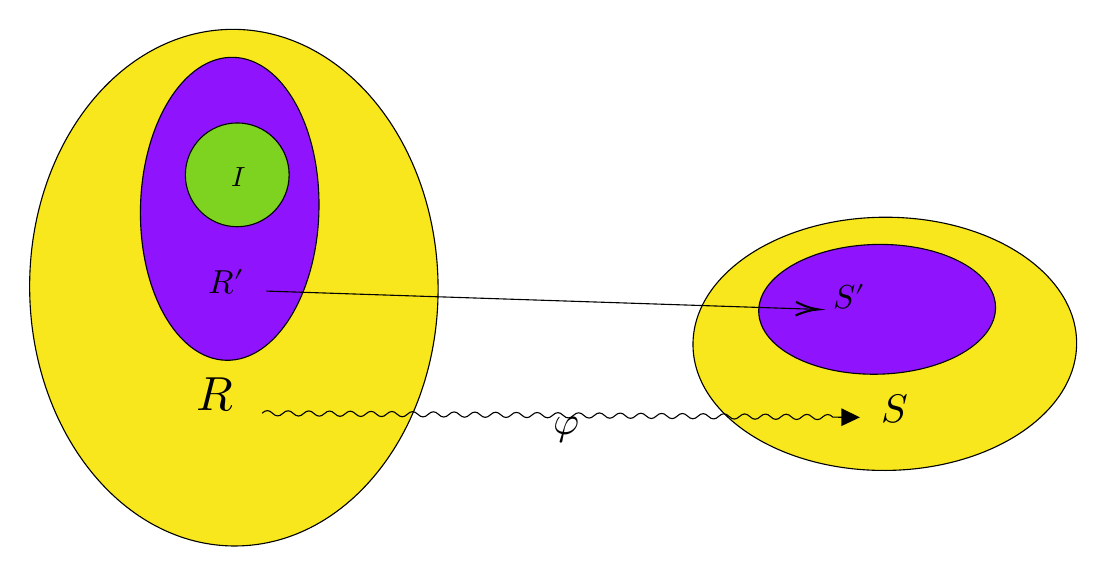
\begin{tikzpicture}[x=0.75pt,y=0.75pt,yscale=-1,xscale=1]
			%uncomment if require: \path (0,300); %set diagram left start at 0, and has height of 300

			%Shape: Ellipse [id:dp6992608779061074] 
			\draw  [fill={rgb, 255:red, 248; green, 231; blue, 28 }  ,fill opacity=1 ] (61.99,147.34) .. controls (61.3,78.6) and (104.8,22.44) .. (159.14,21.9) .. controls (213.47,21.36) and (258.08,76.65) .. (258.76,145.38) .. controls (259.45,214.12) and (215.95,270.27) .. (161.61,270.81) .. controls (107.27,271.36) and (62.67,216.07) .. (61.99,147.34) -- cycle ;
			%Shape: Ellipse [id:dp8268210443202992] 
			\draw  [fill={rgb, 255:red, 248; green, 231; blue, 28 }  ,fill opacity=1 ] (473.66,112.42) .. controls (524.7,112.13) and (566.23,139.21) .. (566.42,172.9) .. controls (566.6,206.59) and (525.38,234.13) .. (474.34,234.42) .. controls (423.3,234.7) and (381.77,207.62) .. (381.58,173.93) .. controls (381.4,140.25) and (422.62,112.7) .. (473.66,112.42) -- cycle ;
			%Straight Lines [id:da3594704358630838] 
			\draw    (174,206.84) .. controls (175.68,205.18) and (177.35,205.19) .. (179,206.87) .. controls (180.65,208.55) and (182.32,208.56) .. (184,206.91) .. controls (185.67,205.26) and (187.34,205.27) .. (189,206.94) .. controls (190.66,208.61) and (192.33,208.62) .. (194,206.97) .. controls (195.68,205.32) and (197.35,205.33) .. (199,207.01) .. controls (200.66,208.68) and (202.33,208.69) .. (204,207.04) .. controls (205.68,205.39) and (207.35,205.4) .. (209,207.08) .. controls (210.66,208.75) and (212.33,208.76) .. (214,207.11) .. controls (215.68,205.46) and (217.35,205.47) .. (219,207.15) .. controls (220.66,208.82) and (222.33,208.83) .. (224,207.18) .. controls (225.68,205.53) and (227.35,205.54) .. (229,207.22) .. controls (230.66,208.89) and (232.33,208.9) .. (234,207.25) .. controls (235.68,205.6) and (237.35,205.61) .. (239,207.29) .. controls (240.66,208.96) and (242.33,208.97) .. (244,207.32) .. controls (245.68,205.67) and (247.35,205.68) .. (249,207.36) .. controls (250.66,209.03) and (252.33,209.04) .. (254,207.39) .. controls (255.68,205.74) and (257.35,205.75) .. (259,207.43) .. controls (260.66,209.1) and (262.33,209.11) .. (264,207.46) .. controls (265.68,205.81) and (267.35,205.82) .. (269,207.5) .. controls (270.66,209.17) and (272.33,209.18) .. (274,207.53) .. controls (275.68,205.88) and (277.35,205.89) .. (279,207.57) .. controls (280.66,209.24) and (282.33,209.25) .. (284,207.6) .. controls (285.67,205.95) and (287.34,205.96) .. (289,207.63) .. controls (290.65,209.31) and (292.32,209.32) .. (294,207.67) .. controls (295.67,206.02) and (297.34,206.03) .. (299,207.7) .. controls (300.65,209.38) and (302.32,209.39) .. (304,207.74) .. controls (305.67,206.09) and (307.34,206.1) .. (309,207.77) .. controls (310.65,209.45) and (312.32,209.46) .. (314,207.81) .. controls (315.67,206.16) and (317.34,206.17) .. (319,207.84) .. controls (320.65,209.52) and (322.32,209.53) .. (324,207.88) .. controls (325.67,206.23) and (327.34,206.24) .. (329,207.91) .. controls (330.65,209.59) and (332.32,209.6) .. (334,207.95) .. controls (335.67,206.3) and (337.34,206.31) .. (339,207.98) .. controls (340.65,209.66) and (342.32,209.67) .. (344,208.02) .. controls (345.67,206.37) and (347.34,206.38) .. (349,208.05) .. controls (350.65,209.73) and (352.32,209.74) .. (354,208.09) .. controls (355.67,206.44) and (357.34,206.45) .. (359,208.12) .. controls (360.65,209.8) and (362.32,209.81) .. (364,208.16) .. controls (365.67,206.51) and (367.34,206.52) .. (369,208.19) .. controls (370.66,209.86) and (372.33,209.87) .. (374,208.22) .. controls (375.68,206.57) and (377.35,206.58) .. (379,208.26) .. controls (380.65,209.93) and (382.32,209.94) .. (383.99,208.29) .. controls (385.67,206.64) and (387.34,206.65) .. (388.99,208.33) .. controls (390.65,210) and (392.32,210.01) .. (393.99,208.36) .. controls (395.67,206.71) and (397.34,206.72) .. (398.99,208.4) .. controls (400.65,210.07) and (402.32,210.08) .. (403.99,208.43) .. controls (405.67,206.78) and (407.34,206.79) .. (408.99,208.47) .. controls (410.65,210.14) and (412.32,210.15) .. (413.99,208.5) .. controls (415.67,206.85) and (417.34,206.86) .. (418.99,208.54) .. controls (420.65,210.21) and (422.32,210.22) .. (423.99,208.57) .. controls (425.67,206.92) and (427.34,206.93) .. (428.99,208.61) .. controls (430.65,210.28) and (432.32,210.29) .. (433.99,208.64) .. controls (435.67,206.99) and (437.34,207) .. (438.99,208.68) .. controls (440.65,210.35) and (442.32,210.36) .. (443.99,208.71) .. controls (445.67,207.06) and (447.34,207.07) .. (448.99,208.75) -- (451,208.76) -- (459,208.82) ;
			\draw [shift={(462,208.84)}, rotate = 180.4] [fill={rgb, 255:red, 0; green, 0; blue, 0 }  ][line width=0.08]  [draw opacity=0] (8.93,-4.29) -- (0,0) -- (8.93,4.29) -- cycle    ;
			%Shape: Ellipse [id:dp6694038570583041] 
			\draw  [fill={rgb, 255:red, 144; green, 19; blue, 254 }  ,fill opacity=1 ] (160.11,35.38) .. controls (183.85,35.94) and (202.32,69.07) .. (201.36,109.38) .. controls (200.4,149.69) and (180.38,181.9) .. (156.64,181.34) .. controls (132.9,180.78) and (114.43,147.64) .. (115.39,107.34) .. controls (116.34,67.03) and (136.36,34.82) .. (160.11,35.38) -- cycle ;
			%Shape: Ellipse [id:dp7396818051441147] 
			\draw  [fill={rgb, 255:red, 144; green, 19; blue, 254 }  ,fill opacity=1 ] (413.25,157.99) .. controls (412.88,140.74) and (438.13,126.2) .. (469.63,125.54) .. controls (501.14,124.87) and (526.98,138.33) .. (527.34,155.58) .. controls (527.7,172.84) and (502.46,187.38) .. (470.95,188.04) .. controls (439.45,188.71) and (413.61,175.25) .. (413.25,157.99) -- cycle ;
			%Straight Lines [id:da5729070577321602] 
			\draw    (176,148) -- (440,156.77) ;
			\draw [shift={(442,156.84)}, rotate = 181.9] [color={rgb, 255:red, 0; green, 0; blue, 0 }  ][line width=0.75]    (10.93,-3.29) .. controls (6.95,-1.4) and (3.31,-0.3) .. (0,0) .. controls (3.31,0.3) and (6.95,1.4) .. (10.93,3.29)   ;
			%Shape: Circle [id:dp5046306025149594] 
			\draw  [fill={rgb, 255:red, 126; green, 211; blue, 33 }  ,fill opacity=1 ] (137,92) .. controls (137,78.19) and (148.19,67) .. (162,67) .. controls (175.81,67) and (187,78.19) .. (187,92) .. controls (187,105.81) and (175.81,117) .. (162,117) .. controls (148.19,117) and (137,105.81) .. (137,92) -- cycle ;

			% Text Node
			\draw (313,207.4) node [anchor=north west][inner sep=0.75pt]  [font=\Large]  {$\varphi $};
			% Text Node
			\draw (158,87.4) node [anchor=north west][inner sep=0.75pt]    {$I$};
			% Text Node
			\draw (141,188.4) node [anchor=north west][inner sep=0.75pt]  [font=\LARGE]  {$R$};
			% Text Node
			\draw (471,196.4) node [anchor=north west][inner sep=0.75pt]  [font=\Large]  {$S$};
			% Text Node
			\draw (147,136.4) node [anchor=north west][inner sep=0.75pt]  [font=\large]  {$R^{\prime }$};
			% Text Node
			\draw (448,143.4) node [anchor=north west][inner sep=0.75pt]  [font=\large]  {$S^{\prime }$};


			\end{tikzpicture}
			\begin{lemma}{}{}
				设$R,S$是两个环,$\varphi : R \rightarrow S$是一个满同态,$I=\ker \varphi$是一个理想

				那么对于包含$I$的任意一个$R$的理想$J$,存在唯一的环同态$\chi : R/J \rightarrow S$,
				
				使得$\varphi =\chi \circ \pi_I$,其中$\pi_I : R \ni a \mapsto a+I \in R/I$
			\end{lemma}

			\begin{them}{同构第二基本定理}{}
				
			\end{them}
	\section{模}
		本节我们研究一种“环上的线性空间”,也就是模
		\subsection{模的定义}
			\begin{defn}{左模}{}
				设$R$是一个环,$M$是一个集合,如果存在两个运算$+ : M \times M \rightarrow M,\cdot_R : R \times M \rightarrow M$
				
				分别称为称为加法和纯量乘法,满足下列条件:

				\ding{172} $\exists 0_M \in M$,称为加法单位元,$\forall \alpha \in M,0_M + \alpha =\alpha +0_M=\alpha $

				\ding{173} $\forall \alpha,\beta  \in M,\alpha +\beta =\beta +\alpha $

				\ding{174} $\forall \alpha,\beta,\gamma  \in M,(\alpha +\beta )+\gamma =\alpha +(\beta +\gamma )$

				\ding{175} $\forall \alpha \in M,\exists -\alpha \in M$,称为加法逆,使得$\alpha +(-\alpha )=0_M$

				\ding{176} $\forall a,b \in R,\alpha \in M,a(b\alpha )=(ab)\alpha$

				\ding{177} $\forall a \in R,\alpha ,\beta \in M,a(\alpha +\beta )=a\alpha +a\beta $

				\ding{178} $\forall a,b \in R,\alpha \in M,(a+b)\alpha =a\alpha +b\alpha $

				那么我们称$M$是一个左$R-$模
			\end{defn}
			类似地,我们也有右模的定义:
			\begin{defn}{右模}{}
				设$R$是一个环,$M$是一个集合,如果存在两个运算$+ : M \times M \rightarrow M,\cdot_R : M \times R \rightarrow M$
				
				分别称为称为加法和纯量乘法,满足下列条件:

				\ding{172} $\exists 0_M \in M$,称为加法单位元,$\forall \alpha \in M,0_M + \alpha =\alpha +0_M=\alpha $

				\ding{173} $\forall \alpha,\beta  \in M,\alpha +\beta =\beta +\alpha $

				\ding{174} $\forall \alpha,\beta,\gamma  \in M,(\alpha +\beta )+\gamma =\alpha +(\beta +\gamma )$

				\ding{175} $\forall \alpha \in M,\exists -\alpha \in M$,称为加法逆,使得$\alpha +(-\alpha )=0_M$

				\ding{176} $\forall a,b \in R,\alpha \in M,(\alpha a)b=\alpha (ab)$

				\ding{177} $\forall a \in R,\alpha ,\beta \in M,(\alpha +\beta )a=\alpha a+\beta b$

				\ding{178} $\forall a,b \in R,\alpha \in M,\alpha (a+b)=\alpha a+\alpha b$

				那么我们称$M$是一个右$R-$模
			\end{defn}
			如果$M$兼具左模和右模的特征,我们称$M$是一个双模:
			\begin{defn}{双模}{}
				如果$M$既是左$R-$模,又是右$S-$模,并且满足:

				$(a \alpha )b=a(\alpha b)$

				那么我们称$M$是一个$(R,S)-$双模
			\end{defn}
			我们也知道,环不一定有乘法单位元,因此有以下定义:
			\begin{defn}{幺模}{}
				设$R$是幺环,$M$是一个$R-$模

				如果$\forall \alpha \in M,1_R \cdot \alpha =\alpha $,那么我们称$M$是一个幺模。
			\end{defn}
			在后续中,除非特别做区分,我们都假定我们说的模指的是左模。
		\subsection{模的同态}
			\begin{defn}{模同态}{}
				设$M,N$是两个$R-$模,如果映射$\psi  : M \rightarrow N$满足:

				$\forall \alpha ,\beta  \in M,\psi (\alpha +\beta )=\psi (\alpha )+\psi (\beta )$

				$\forall a \in R,\alpha  \in M,\psi (a\alpha )=a\psi (\alpha )$

				那么称$\psi $是一个从$M$到$N$的模同态。
			\end{defn}
		\subsection{商模}
			\begin{defn}{商模}{}
				设$M$是一个模,$N$是$M$的一个子模
			\end{defn}
\ifx\allfiles\undefined
\end{document}
\fi